\begin{problem}
Given a circle centered at $O$, there exists an obtuse triangle $ABC$ inscribed in the circle such that $B$ is obtuse. If $AB=3$ and $BC=8$, and the height from $B$ to $\overline{AC}$ is $2$, the area of the circle can be written as $n\pi$. Find $n$.
\end{problem}

\begin{solution}
Let $h$ be the length of the height from $B$ to $\overline{AC}$. Then, by similarity, $AB:h=2R:BC$. Hence, $AB(BC)=h(2R)$. Thus, $24=4R$. The radius is $4$, so the area of the circle equals $16\pi$. The answer is $16$.
\end{solution}

\begin{problem}
Determine the remainder when $3^{15}+5^{15}$ is divided by $17$. 
\end{problem}

\begin{solution}
According to Fermat's Little Theorem, $3^{16}\equiv 5^{16} \equiv 1 \pmod{17}$.
\begin{align*}
    3^{15}+5^{15} & \equiv \frac13+\frac15 \pmod{17}\\
    & \equiv \frac{18}{3}+\frac{35}{5} \pmod{17}\\
    & \equiv 6+7 \pmod{17}\\
    & \equiv 13 \pmod{17}
\end{align*}
The answer is $13$.
\end{solution}

\begin{problem}
Given positive real numbers $a$, $b$, $c$, and $d$, if $(a+c)(b+d)=121$, determine the least value of $a+b+c+d$.
\end{problem}

\begin{solution}
According to AM-GM inequality, 
\begin{align*}
    \dfrac{(a+c)+(b+d)}{2} & \geq \sqrt{(a+c)(b+d)}\\
    \dfrac{a+b+c+d}{2} & \geq \sqrt{121}\\
    a+b+c+d &\geq 2(11)\\
    &\geq 22
\end{align*}
The answer is $22$.
\end{solution}

\begin{problem}
Given three positive integers $a>b>c\geq1$, let $N$ be the number of triples $(a,b,c)$ such that $a+b+c=331$. Find the last three digits of $N$.
\end{problem}

\begin{solution}
Stars-and-bars imply that the total number of triples without condition equals $\binom{333}{2}$. Assume that $a=b>c$. Then, $2a+c=331$. Diophantine equation shows $166$ triples. Arrange $166$ triples by $\frac{3!}{2!}=3$ ways. Hence, subtract $498$ from $55278$ to retrieve $54780$. The answer is $780$.
\end{solution}

\begin{problem}
Compute the number of sequences that are arrangements of the numbers $1$, $2$, $3$, $4$, and $5$ and satisfy the requirement that no term in the sequence is larger than or equal to the square of the next term.
\end{problem}

\begin{solution}
First, $1$ should stay in the front of the sequence. Notice that $1<2^2$, $3<2^2$ and $4=2^2$. Hence, we only allow $12$ or $32$ as two consecutive terms in the sequence. Arrange $3$, $4$, and $5$, in $3!(=6)$ ways. Then, place $2$ next to either $1$ or $3$, in $2!(=2)$ ways. Therefore, there are $12$ sequences satisfying the given condition. The answer is $12$.
\end{solution}

\begin{problem}
Determine the number of ordered pairs of positive integers $(a,b)$ such that $a^b=3^{3^3}$.
\end{problem}

\begin{solution}
Since $3^{3^3}$ is $3^{27}$. there is one-to-one correspondence between the number of divisors of $27$ and $(a,b)$. Hence, there are $4$ pairs of $(a,b)$. The answer is $4$.
\end{solution}

\begin{problem}
Compute the least positive integer value of $n$ such that $10n$ and $12n$ have the same number of divisors.
\end{problem}

\begin{solution}
Let $n=2^a3^b5^c$. $10n$ and $12n$ have the equal number of divisors if and only if $(a+2)(b+1)(c+2)=(a+3)(b+2)(c+1)$. The smallest value of $n$ can be retrieved when $a=0$, $b=2$ and $c=0$. Thus, the answer is $9$.
\end{solution}

\begin{problem}
On the complex plane there are six complex numbers satisfying $z^6=1$. Given that $z$, $z^2$ and $z^3$ form a non-degenerate triangle, the ratio between the smallest area and largest area formed by $z$, $z^2$ and $z^3$ can be written as $\frac{a}{b}$ where $a$ and $b$ are relatively prime integers. Find $a+b$.
\end{problem}

\begin{solution}
The smallest area is $\frac{\sqrt{3}}{4}$, whereas the largest area is $\frac{3\sqrt{3}}{4}$. Hence, the ratio equals $\frac{1}{3}$. The answre is $4$.
\end{solution}

\begin{problem}
Three customers in a grocery store saw there are five apples and four oranges. After they left, there was no lemon nor orange left. In how many ways would the customers buy these fruits such that each takes at least one fruit of ANY type?
\end{problem}

\begin{solution}
There are $315$ number of ways to distribute fruits to these customers. Apply De Morgan's Law and Principle of Inclusion and Exclusion. There are $87$ bad ways such that there is at least one person not buying any fruit. Hence, the answer is $228$.
\end{solution}

\begin{problem}
Determine the sum of $x$-intercepts of a graph of $f(x)=(x-2)^7-x^7-4$.
\end{problem}

\begin{solution}
The graphs of two functions $y=(x-2)^7$ and $y=x^7+4$ intersect at two real points. Let $x=r$. then, $x=2-r$ is also the real solution. Hence, the sum of two real $x$-intercepts equals $2$. The answer is $2$.
\end{solution}

\begin{problem}
Suppose $f(x)=x^3-x+1$ has roots $r$, $s$, and $t$. Determine $\frac{r^3}{r-1}+\frac{s^3}{s-1}+\frac{t^3}{t-1}$.
\end{problem}

\begin{solution}
According to Viete's formula, $f(r)=f(s)=f(t)=0$. Hence, $r^3=r-1$, $t^3=t-1$ and $s^3=s-1$. The answer is $3$. 
\end{solution}

\begin{problem}
Determine the maximum possible value of $xy$ if $x^2+5xy+y^2=1001$ for real $x$ and $y$.
\end{problem}

\begin{solution}
According to AM-GM inequality, $x^2+5xy+y^2\geq 7xy$. Hence, $xy\leq 143$. Check that $x=y=\sqrt{143}$. The answer is $143$.
\end{solution}

\begin{problem}
The sum $\sum_{k=2}^{100}\frac{1}{\binom{k}{2}}$ can be written as $\frac{m}{n}$ where $m$ and $n$ are relatively prime positive integers. Find $m+n$.
\end{problem}

\begin{solution}
This telescopes so the sum changes into $2(1-\frac{1}{101})=\frac{200}{101}$. The answer is $301$.
\end{solution}

\begin{problem}
There are three rows with three seats each. If Mary, May and Mo wish to sit down, in how many ways can they be seated in different rows and different columns?
\end{problem}

\begin{solution}
Send Mary, May, and Mo, in that order. The answer is $36$.
\end{solution}

\begin{problem}
In how many ways can four $($'s and $)$'s be arranged in a line such that $)$ must be written after $($?
\end{problem}

\begin{solution}
This is a typical Catalan number problem for $4\times4$. Hence, there are $\frac{1}{5}\binom{8}{4}=14$. The answer is $14$.
\end{solution}

\begin{problem}
Points $P$ and $Q$ lie outside and inside square $AIME$, respectively such that $\triangle API \cong \triangle MQI$ and $m\angle API = 90^\circ$. Suppose that $AP=1$ and $PQ=24$. Compute $[AIME]$ where $[AIME]$ refers to the area of $\square AIME$.
\end{problem}

\begin{solution}
Apply Pythagorean Theorem to conclude that $PI=12\sqrt{2}$ and $AP=1$, so $AI=17$. Hence, $AI^2=289=[AIME]$. The answer is $289$.
\end{solution}

\begin{problem}
A polynomial equation $x^3+px^2+12x+q=0$ has integer roots, one of which is $1$. Find the maximal possible value of $p$.
\end{problem}

\begin{solution}
According to Viete's formula, let $x^3+px^2+12x+q=(x-1)(x-a)(x-b)$ for two other solutions $a$ and $b$. Then, $(a+1)(b+1)=13$ implies that $(a,b)=(12,0)$, $(0,12)$, $(-14,-2)$ and $(-2,-14)$. Hence, $p=-a-b-1$ is either $15$ or $-13$. The largest possible value is $15$. The answer is $15$.
\end{solution}

\begin{problem}
Let $n$ be the number of degree $5$ polynomials $f(x)$ with non-negative integer coefficients such that $f(1)=10$ and $f(-1)=4$. Find the total possible number of $f(x)$s.
\end{problem}

\begin{solution}
Apply stars and bars twice to get $216(=36\times6)$ polynomials of $x$. The answer is $216$.
\end{solution}

\begin{problem}
Eunchan and Joochan made unit cubes, respectively, using magnetic balls and sticks. They decided to use all to make a new right prism, using all of the sticks and balls. They found out each of the faces is regular polygon. The volume of the new prism can be written as $a+\sqrt{b}$. Find $a+b$.
\end{problem}

\begin{solution}
This new solid is an octagonal prism. The base area equals $2+2\sqrt{2}$, and the height equals $1$. Hence, the volume equals $2+\sqrt{8}$. The answer is $10$.
\end{solution}

\begin{problem}
Three standard, fair six-sided die are rolled at a time. Given that the sum of the values rolled is $12$, the probability that at least two of the shown values is prime can be written as $\frac{m}{n}$ for relatively prime $m$ and $n$. Find $m+n$.
\end{problem}


\begin{solution}
\begin{align*}
a+b+c&=12\\
6+5+1&=12\\ 
6+4+2&=12\\
6+3+3&=12\\ 
5+5+2&=12\\ 
5+4+3&=12\\ 
4+4+4&=12
\end{align*}
Out of $216$ triples, there are $12$ triples satisfying this property. Hence, $\frac{12}{216}=\frac{2}{36}=\frac{1}{18}$. Hence, the answer is $19$.
\end{solution}

\begin{problem}
Determine the remainder when $111,111,111,111$ is divided by $17$.
\end{problem}

\begin{solution}
The answer is $7$.
\end{solution}

\begin{problem}
If four fair six-sided die are rolled, the probability that the average of four outcomes is $3$ can be written as $\frac{m}{n}$ where $m$ and $n$ are relatively prime positive integers. Determine $m+n$.
\end{problem}

\begin{solution}
The answer is $1421$.
\end{solution}

\begin{problem}
Given a right isosceles triangle $ABC$ where $AB=BC=3$ and $AC=3\sqrt{2}$, the probability that a point inside the triangle is closer to $AC$ than to either $AB$ or $BC$ can be written as $\sqrt{a}-b$ where $a$ and $b$ are positive integers, and $a$ is a square-free integer. Determine $a+b$.
\end{problem}

\begin{solution}
The answer is $3$.
\end{solution}

\begin{problem}
Suppose $\overline{AB}$ and $\overline{BC}$ are the chords of the same circle centered at $O$ such that their perpendicular bisectors meet at $O$. If $AB=4$ and $BC=7$, then the area of circle can be written as $\frac{a\pi}{b}$ where $a$ and $b$ are relatively prime positive integers. Determine the value of $ab$.
\end{problem}

\begin{solution}
The answer is $260$.
\end{solution}

\begin{problem}
If four fair six-sided die are rolled, the probability that the four outcomes, possibly rearranged if necessary, form an arithmetic sequence allowing the common difference of $0$, can be written as a reduced fraction $\frac{m}{n}$ where $m$ and $n$ are relatively prime positive integers. Determine the value of $m$.
\end{problem}

\begin{solution}
The answer is $13$.
\end{solution}

\begin{problem}
Two circles of different radii are tangent at a point $P$. If an external tangent to two circles meets the internal tangent line passing through $P$ at a point $Q$. Find $PQ^2$ if two radii are $7$ and $3$, respectively.
\end{problem}

\begin{solution}
The answer is $21$.
\end{solution}

\begin{problem}
Determine the sum of the digits of $111,111,111^2$.
\end{problem}

\begin{solution}
The answer is $81$.
\end{solution}

\begin{problem}
Given a right triangle with side lengths $6$, $8$, and $10$, if $H$ is the orthocenter, $O$ is the circumcenter, let $P$ be the midpoint of $\overline{OH}$. If $G$ is the centroid of the triangle, then the length of $PG$ can be written as $\frac{m}{n}$ where $m$ and $n$ are relatively prime positive integers. Determine $m+n$.
\end{problem}

\begin{solution}
The answer is $11$.
\end{solution}

\begin{problem}
Given a quadrilateral $ABCD$ where $AB=8$, $BC=6$, $CD=5\sqrt{2}$ and $AD=5\sqrt{2}$, if $\angle B$ and $\angle D$ are right angles, then $BD$ can be written as $a\sqrt{b}$ where $a$ and $b$ are positive integers, and $b$ is a square-free. Determine $a+b$.
\end{problem}

\begin{solution}
The answer is $9$.
\end{solution}

\begin{problem}
For a $4$-digit positive integer $n$, if $n^2$ and $n$ has the same remainder when divided by $100$, find the number of all such $n$ satisfying the given condition.
\end{problem}

\begin{solution}
The answer is $360$.
\end{solution}

\begin{problem}
Determine the smallest positive integer $n$ such that $n!$ end with exactly $10$ zeros.
\end{problem}

\begin{solution}
The answer is $45$.
\end{solution}

\begin{problem}
If $20a+23b=2023$ for non-negative integers $a$ and $b$, determine the total number of $(a,b)$ pairs satisfying the given equation.
\end{problem}

\begin{solution}
The answer is $5$. Here is one way of solving the problem.\\
	Let $a$ and $b$ be non-negative integers satisfying $20a+23b=2023$. Then,
	\begin{align*}
		20a+23b&=2023\\
		0a+3b&\equiv 3 \pmod{20}\\
		3b&\equiv 3 \pmod{20}\\
		b&\equiv 1 \pmod{20}
	\end{align*}
	Hence, $b=20k+1$ for some integer $k$. Since $23b=2023-20a\leq 2023$, we set $b\leq 87\frac{22}{23}$. Hence, $20k+1 \leq 87\frac{22}{23}$ implies that $0\leq k \leq 4$. Thus, there are $5$ values of $k$.
\end{solution}

\begin{problem}
Given a monic cubic polynomial equation $x^3-5x^2+7x-11=0$ with solutions $r$, $s$, and $t$, determine the exact value of $r^3+s^3+t^3$.
\end{problem}

\begin{solution}
The answer is $53$. Here is one way of solving the problem. Let $r$, $s$, and $t$ be the solutions to the given polynomial equation. Then, by Viete's formula,
	\begin{align*}
		x^3-5x^2+7x-11 &= (x-r)(x-s)(x-t)\\
		x^3-5x^2+7x-11 &= x^3-(r+s+t)x^2+(rs+st+tr)x-rst
	\end{align*}
	Thus, we conclude that $r+s+t=5$, $rs+st+tr=7$ and $rst=11$.\\
	\bigskip
	According to algebraic identity of cubic sums, we get
	\begin{align*}
	r^3+s^3+t^3-3rst &= (r+s+t)(r^2+s^2+t^2-rs-st-tr)\\
	r^3+s^3+t^3 &= (r+s+t)(r^2+s^2+t^2-rs-st-tr)+3rst\\
	&= (r+s+t)((r+s+t)^2-3(rs+st+tr))+3rst\\
	&=5((5^2)-3(7))+3(11)\\
	&=20+33\\
	&=53
	\end{align*}
	Another way to solve this problem is to use Newton's Identity. Let $S_1=r+s+t$, $S_2= r^2+s^2+t^2$, and $S_3=r^3+s^3+t^3$. Then, by Newton's identity,
	\begin{align*}
		S_1-5(1)&=0\\
		S_2-5S_1+7(2)&=0\\
		S_3-5S_2+7S_1-11(3)&=0
	\end{align*}
	Hence, $S_1=5$, $S_2=11$, and $S_3=53$.
\end{solution}

\begin{problem}
For a quadratic function $f(x)=x^2-2$, for real $(x,y)$, if $|x|+2|y|\leq2$, then the minimum possible value of $f(x)$ can be written as $\frac{-a+\sqrt{b}}{c}$ where $a$, $b$, and $c$ are positive integers, and $b$ is a square-free integer. Determine the sum $a+b+c$. (Terminology: a square-free integer is a positive integer that is not divisible by any perfect square (other than 1).)
\end{problem}

\begin{solution}
The answer is $32$.\\
	\begin{center}
	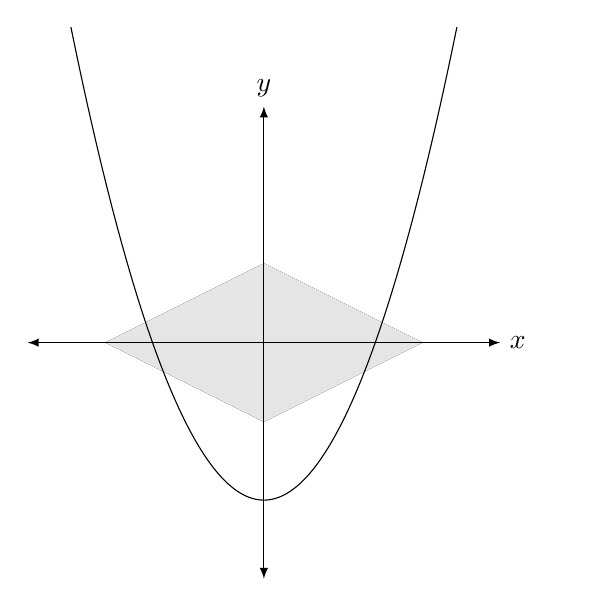
\begin{tikzpicture}
		% Set the limits of the x and y axes
		\def\xmin{-3}
		\def\xmax{3}
		\def\ymin{-3}
		\def\ymax{3}
		
		\clip (\xmin,\ymin) rectangle (\xmax+1,\ymax+1);
		
		\draw  (-2,0)--(0,1)--(2,0)--(0,-1)--cycle;
		\filldraw[gray!20] (-2,0)--(0,1)--(2,0)--(0,-1)--cycle;
		
		% Draw the graph of y = x^2 - 2
		\draw[domain=\xmin:\xmax, smooth, samples=100] plot (\x,{\x*\x - 2});
		\draw[latex-latex] (\xmin,0) -- (\xmax,0) node[right] {$x$};
		\draw[latex-latex] (0,\ymin) -- (0,\ymax) node[above] {$y$};
	\end{tikzpicture}
	\end{center}
As one can see from the figure above, $x^2-2=\frac{1}{2}x-1$ or $x^2-2=-\frac{1}{2}x-1$ result in the minimum possible value of $f(x)$. Hence, solving the equations, we get either $2x^2-4=x-2$ or $2x^2-4=-x-2$. Since $2x^2-x-2=0$ or $2x^2+x-2=0$, we get $x=\frac{1-\sqrt{15}}{4}$ or $\frac{-1+\sqrt{15}}{4}$.\\
\bigskip
The first solution will result in 
\begin{align*}
	y=-\frac{1}{2}x-1=-\frac{1}{2}\left(\frac{1-\sqrt{15}}{4}\right)-1=\frac{-9+\sqrt{15}}{8}
\end{align*}
Similarly, the second solution will result in 
\begin{align*}
	y=\frac{1}{2}x-1=\frac{1}{2}\left( \frac{-1+\sqrt{15}}{4} \right) -1 = \frac{-9+\sqrt{15}}{8}
\end{align*}
Hence, $a=9$, $b=15$, and $c=8$. Thus, $a+b+c=9+15+8=32$.\\
\end{solution}

\begin{problem}
Given an equilateral triangle $ABC$ of side length $6$, suppose there is a square $PQRS$ inside the triangle such that three of its vertices are on the sides of the square, i.e., $\overline{AB}$, $\overline{BC}$, $\overline{AC}$. If $P$ is on the midpoint of $\overline{BC}$, $Q$ and $S$ are on $\overline{AB}$ and $\overline{AC}$, respectively, then $QS=a-b\sqrt{c}$ if $A$, $R$, and $P$ are collinear. If $a$, $b$, and $c$ are positive integers such that $c$ is a square-free integer, determine the product $abc$.\\
\end{problem}

\begin{solution}
The answer is $81$. It is clear that $m\angle QPB = m \angle SPC = 45^\circ$, since $A$, $R$, and $P$ are collinear. Let $O$ be the intersection point between $\overline{QS}$ and $\overline{AP}$. Then, we may label $QO=RO=SO=OP=k$. This implies that 
\begin{align*}
	BQ&=\frac{2k}{\sqrt{3}}=\frac{2\sqrt{3}k}{3}\\
	AQ&=6-\frac{2\sqrt{3}k}{3}
\end{align*}
Since $AQS$ is an equilateral triangle, we may use $\frac{AQ}{OQ}=\frac{1}{2}$. Hence, $\frac{6-\frac{2\sqrt{3}k}{3}}{k}=\frac{1}{2}$. Thus, $k=\frac{9-3\sqrt{3}}{2}$. Since $QS=PR=2k$, we conclude that $QS=a-b\sqrt{c}=9-3\sqrt{3}$. Thus, $a=9$, $b=3$, and $c=3$. Therefore, $abc=9\cdot3\cdot3=81$.\\
\bigskip
Similarly, if we use the laws of sines, 
\begin{align*}
	\frac{QP}{BP}&=\frac{k\sqrt{2}}{3}\\
	&=\frac{\sin(60^\circ)}{\sin(75^\circ)}\\
	&=\frac{\sqrt{3}/2}{(\sqrt{6}+\sqrt{2})/4}\\
	&=\frac{2\sqrt{3}}{\sqrt{6}+\sqrt{2}}
\end{align*}
Hence, $k=\frac{36-12\sqrt{3}}{8}$. Thus, $2k=QS=9-3\sqrt{3}$. Hence, $abc=81$.
\end{solution}

\begin{problem}
Given a piece-wise function $f(x)$ defined on $0\leq x \leq 2$ and $0\leq y \leq 2$ such that
$$\begin{cases} x+1 & (0\leq x < 1) \\ 4-2x & (1\leq x \leq 2) \end{cases},$$ the graph of $y=f(f(f(x)))$, the $x$-axis and the vertical line $x=2$ form a bounded region. The area of the bounded region can be written as $\frac{m}{n}$ where $m$ and $n$ are relatively prime positive integers. Determine $m+n$.
\end{problem}

\begin{solution}
The answer is $27$. Students learn sketching the graph of composition of functions in the first semester of Precalculus or second semester of Algebra 2. The graph of $y=f(f(f(x)))$ is given by the following figure.
\begin{center}
	\begin{tikzpicture}[scale=1.5]
		\draw[-latex] (-0.5,0)--(3,0);
		\draw[-latex] (0,-0.5)--(0,3);
		\draw[dotted] (2,0)--(2,2)--(0,2);
		\draw (0,0)--(0.5,2)--(1,1)--(1.25,2)--(1.5,0)--(2,2);
		\draw (0.5,2)--(0.5,0) [dotted];
		\draw (0,1)--(1,1)--(1,0) [dotted];
		\draw (1.25,2)--(1.25,0) [dotted];
		\node[below] at (0.5,0) {$\frac12$};
		\node[below] at (1,0) {$1$};
		\node[below] at (1.25,0) {$\frac54$};
		\node[below] at (1.5,0) {$\frac32$};
		\node[below] at (2,0) {$2$};
		\node[left] at (0,2) {$2$};
		\node[left] at (0,1) {$1$};
		\node[right] at (3,0) {$x$};
		\node[above] at (0,3) {$y$};
	\end{tikzpicture}
\end{center} 
Hence, the area bounded by the graph of $y=f(f(f(x)))$, the $x$-axis, and the vertical line $x=2$ can be computed as 
\[
\frac12+\frac34+\frac38+\frac14+\frac12=2+\frac38=\frac{19}{8}
\]
Thus, $m=19$ and $n=8$. The sum of $m$ and $n$ is $27$.\\
\end{solution}

\begin{problem}
Given a set of integers $\{1,2,3,4,5,6,7,8,9\}$, if five integers, not necessarily distinct, are chosen at random, as $a$, $b$, $c$, $d$, and $e$, respectively, the probability that $a\leq b < c \leq d \leq e$ can be written as $\frac{m}{n}$ where $m$ and $n$ are relatively prime positive integers. Determine the exact value of $m$. (In this problem, make sure that $b<c$.)
\end{problem}

\begin{solution}
The answer is $88$. We perform caseworks.
\begin{enumerate}
	\item $a=b<c=d=e$ implies that there are $\binom{9}{2}$ choices for $(a,b,c,d,e)$.
	\item $a<b<c=d=e$ implies that there are $\binom{9}{3}$ choices for $(a,b,c,d,e)$.
	\item $a<b<c<d=e$ implies that there are $\binom{9}{4}$ choices for $(a,b,c,d,e)$.
	\item $a<b<c<d<e$ implies that there are $\binom{9}{5}$ choices for $(a,b,c,d,e)$.
	\item $a=b<c<d<e$ implies that there are $\binom{9}{4}$ choices for $(a,b,c,d,e)$.
	\item $a=b<c=d<e$ implies that there are $\binom{9}{3}$ choices for $(a,b,c,d,e)$.
	\item $a=b<c<d=e$ implies that there are $\binom{9}{3}$ choices for $(a,b,c,d,e)$.
	\item $a<b<c=d<e$ implies that there are $\binom{9}{4}$ choices for $(a,b,c,d,e)$.
\end{enumerate}
Hence, we use the hockey-stick identity to compute the following expression, i.e.,
\begin{align*}
	&\binom92+\binom93+\binom94+\binom95+\binom94+\binom93+\binom93+\binom94\\
	&= \binom{10}{3}+\binom{10}{5}+\binom{10}{4}+\binom{10}{4}\\
	&=\binom{11}{4}+\binom{11}{5}\\
	&=\binom{12}{5}
\end{align*}
Thus, the probability $\frac{m}{n}$ is equivalent to $\frac{11\cdot9\cdot8}{9\cdot9\cdot9\cdot9\cdot9}=\frac{88}{6561}$. Hence, $m=88$.
\end{solution}

\begin{problem}
Given a regular pentagon cut into five congruent triangles with their common vertices in the middle of the figure, Bob is coloring each triangle with three different pastes - blue, red or orange - allowing repetitions. Determine the number of distinct pentagon colorings such that blue triangles must not be adjacent to red ones, if any.
\end{problem}

\begin{solution}
The answer is $83$. We may use recursion and tree diagram. If the first region is colored with blue, then the second region can be colored either blue or orange. Likewise, if the first region is colored with red, then the second region can be colored either red or orange. On the other hand, if the first region is colored with orange, then the second region can be colored either blue, red, or orange.\\
\bigskip
If we begin coloring the first region by blue, then the fifth region can be colored with some pastes, according to the given condition can be counted as $29$, in total. However, since the fifth region cannot be colored as red, we must eliminate all red regions that occurred in the fifth region-coloring. Hence, there are $21$ possible ways to color the fifth region, still satisfying the given condition.\\
\bigskip
Likewise, if we begin coloring the first region by red, the symmetric counting implies that there are $21$ possible colorings of the fifth region.\\
\bigskip
On the other hand, if we begin coloring the first region by orange, then there are $41$ ways to color the fifth region, using the basic recursive form. Since there is no limitation on orange, we keep all $41$ colorings as valid counts. Hence, we take the sum of all possible colorings as $21+21+41=83$.\\ 
\end{solution}

\begin{problem}
Given a positive $9$-digit integer such that there are three $2$'s, three $4$'s and three $0$'s, determine the total number of positive $9$-digit integers divisible by $12$.
\end{problem}

\begin{solution}
The answer is $770$. The sum of all $9$ digits is already divisible by $3$ by default. Hence, we perform caseworks for divisibility by $4$.\\
\begin{enumerate}
	\item If the last two digits are $00$, then there are $\binom{7}{3,3}-\binom{6}{3,3}=120$ number of ways to arrange the remaining digits for $9$-digit integer.
	\item If the last two digits are $20$, then there are $\binom{7}{3,2,2}-\binom{6}{2,3}=150$ number of ways to arrange the remaining digits for $9$-digit integer.
	\item If the last two digits are $24$, then there are $\binom{7}{3,2,2}-\binom{6}{2,2,2}=120$ number of ways to arrange the remaining digits for $9$-digit integer.
	\item If the last two digits are $40$, then there are $\binom{7}{3,2,2}-\binom{6}{3,2}=150$ number of ways to arrange the remaining digits for $9$-digit integer.
	\item If the last two digits are $44$, then there are $\binom{7}{3,3}-\binom{6}{3,2}=80$ number of ways to arrange the remaining digits for $9$-digit integer.
	\item If the last two digits are $04$, then there are $\binom{7}{3,2,2}-\binom{6}{3,2}=150$ number of ways to arrange the remaining digits for $9$-digit integer.
\end{enumerate}
Hence, there are $770$ positive $9$-digit integers divisible by $12$.
\end{solution}

\begin{problem}
There is a closed region formed by connecting $(232023,232023)$, $(232019,232014)$, $(232022, 232022)$,  $(232014,232019)$, and back to $(232023,232023)$, in the written order. Determine the area of closed region.
\end{problem}

\begin{solution}
The answer is $5$. Since the area of the figure will not change under translation, we translate all the points by applying $$(x',y')=(x-232014,y-232014).$$ Have a look at the following figure. 
\begin{center}
	\begin{tikzpicture}[scale=0.7]
		\draw (0,0)--(9,0)--(9,9)--(0,9)--cycle [dotted];
		\draw (0,5)--(9,9)--(5,0)--(8,8)--cycle;
		\node[left] at (0,5) {$(0,5)$};
		\node[below left] at (0,0) {$(0,0)$};
		\node[below] at (5,0) {$(5,0)$};
		\node[above] at (9,9) {$(9,9)$};
		\node[right] at (10,8) {$(8,8)$}; 
		\draw[latex-] (8,8)--(10,8) [dotted];
		\filldraw (5,0) circle (2pt);
		\filldraw (0,5) circle (2pt);
		\filldraw (8,8) circle (2pt);
		\filldraw (9,9) circle (2pt);
	\end{tikzpicture}
\end{center}
The shoelace theorem suggests that 
\[
\text{Area}= \frac{1}{2}|(9\cdot5+0\cdot8+8\cdot0+5\cdot9)-(9\cdot0+5\cdot8+8\cdot5+0\cdot9)| = \frac{1}{2} |10| = 5
\]
\end{solution}

\begin{problem}
Given a square $ABCD$ of side length $4$, a special laser point is shot from $A$ to a point $P_1$ on $\overline{BC}$ such that $AB:BP_1=4:1$. This laser is so special that it reflects to a point $P_2$ on $\overline{CD}$ such that $AP_1P_2$ is a right angle. Then, a laser will be shot to a point $P_3$ on $\overline{AD}$ such that $P_1P_2P_3$ is right. This process continued until there are $P_1$ on $\overline{BC}$, $P_2$ on $\overline{CD}$, $P_3$ on $\overline{AD}$ and $P_4$ on $\overline{AP_1}$. The area of $P_1P_2P_3P_4$ can be written as $\frac{m}{n}$ where $m$ and $n$ are relatively prime positive integers. Determine $m+n$.
\end{problem}

\begin{solution}
The answer is $727$. Let's draw a figure, focusing on the similar triangles. 
\begin{center}
	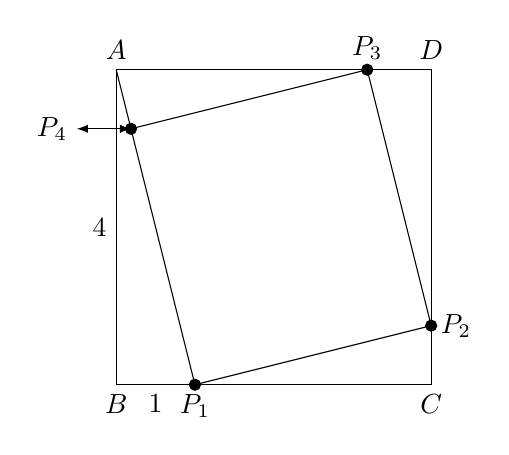
\begin{tikzpicture}
		\draw (0,0)--(4,0)--(4,4)--(0,4)--cycle;
		\draw (0,4)--(1,0)--(4,3/4)--(51/16,4)--(3/16,13/4);
		\node[left] at (0,2) {$4$};
		\node[below] at (0.5,0) {$1$};
		\node[below] at (1,0) {$P_1$};
		\node[right] at (4,3/4) {$P_2$};
		\node[above] at (51/16,4) {$P_3$};
		\node[left] at (-0.5,13/4) {$P_4$};
		\draw[latex-latex] (-0.5,13/4)--(3/16,13/4);
		\filldraw (1,0) circle (2pt);
		\filldraw (4,3/4) circle (2pt);
		\filldraw (51/16,4) circle (2pt);
		\filldraw (3/16, 13/4) circle (2pt);
		\node[above] at (0,4) {$A$};
		\node[below] at (0,0) {$B$};
		\node[below] at (4,0) {$C$};
		\node[above] at (4,4) {$D$};
	\end{tikzpicture}
\end{center}
Since $CP_1:CP_2=4:1$, it is easy to find out $CP_2=\frac34$. Hence, $P_1P_2=\frac{3\sqrt{17}}{4}$. Since $P_2D=\frac{13}{4}$, the similar triangle ratio implies that $P_2P_3=\frac{13\sqrt{17}}{16}$. Thus, the area of $P_1P_2P_3P_4$ can be computed as the area of rectangle, i.e., 
\[
\frac{3\sqrt{17}}{4}\times\frac{13\sqrt{17}}{16}=\frac{39\cdot17}{64}=\frac{663}{64}
\]
Hence, $m+n=663+64=727$.
\end{solution}

\begin{problem}
Given a real valued function $f(x)=\{x\}=x-\lfloor x \rfloor$, where $\lfloor x \rfloor$ is the greatest integer less than or equal to $x$, and $g(x)=\sin(2\pi x)$, let $h(x)=f(g(x))$. Then, there exist $n$ number of solutions satisfying $h(h(x))=x$. Determine the exact value of $n$.
\end{problem}

\begin{solution}
The answer is $16$. In particular, at $0\leq x \leq \frac14$, the value of $h(x)$ shifts from $0$ to $1$, meaning that $h(h(x))$ must graph the full portion of $y=h(x)$ squeezed inside the interval $[0,\frac14]$. At $\frac14\leq x \leq \frac12$, the value of $h(x)$ shifts from $1$ to $0$, meaning that $h(h(x))$ must graph the full portion of $y=h(x)$ in reverse direction inside the given interval. We perform such graphing skill-sets in order to graph $y=h(h(x))$. Hence, we directly compute the number of intersections between $y=h(h(x))$ and $y=x$ as $16$ different points.
\end{solution}

\begin{problem}
Determine the exact value of \[\left(\cos(\frac{2\pi}{2023})+\cos(\frac{4\pi}{2023})+\cos(\frac{6\pi}{2023})+\cdots+\cos(\frac{4044\pi}{2023})\right)^2.\]
\end{problem}

\begin{solution}
The answer is $1$. Notice that $z^{2023}=1$ produces $2023$ roots of unity such that $z_{k}=\cos(\frac{2\pi k}{2023})+i\sin(\frac{2\pi k}{2023})$ for $k=0,1,2,\cdots,2022$ is a unique solution to the given equation. Now, have a look at $z^{2023}-1=0$. The sum of solutions must be $0$ by Viete's formula. In other words, 
$$
(\cos(0)+\cos(\frac{2\pi}{2023})+\cdots+\cos(\frac{4044\pi}{2023}))+i(\sin(0)+\sin(\frac{2\pi}{2023})+\cdots+\sin(\frac{4044\pi}{2023}))= 0+0i
$$
Hence, $\cos(\frac{2\pi}{2023})+\cos(\frac{4\pi}{2023})+\cdots+\cos(\frac{4044\pi}{2023})=-1$. Thus, $(-1)^2=1$.
\end{solution}

\begin{problem}
Let $ABCD$ be a parallelogram such that $m\angle B <90^\circ$ and $AB<BC$. Let $H$ be the intersection point between the altitude from $A$ to $\overline{BC}$ and the altitude from $C$ to $\overline{AB}$. Let $P$ and $Q$ be the perpendicular foot from $A$ to $\overline{BC}$ and from $C$ to $\overline{AB}$, respectively. If $QH:AH:PH=1:3:4$, then $\tan^2(\angle HDC)$ can be written as $\frac{m}{n}$ where $m$ and $n$ are relatively prime positive integers. Determine $m+n$.
\end{problem}

\begin{solution}
The answer is $177$. Let $AH=3k$, $QH=k$, and $PH=4k$. Then, by similar triangles formed by orthocenter, it is easy to find out that $CH=12k$ and $AB=\frac{21\sqrt{8}}{8}k$. Since $Q$ is the perpendicular foot from $C$ to $\overline{AB}$, it is clear that $\angle DCH$ is right. Hence, $\tan(\angle HDC)$ can be written as $\frac{CH}{CD}$. Since $CH=12k$ and $CD=AB=\frac{21\sqrt{8}}{8}k$, we conclude that
\begin{align*}
	\tan(\angle HDC)&=\dfrac{12k}{21\sqrt{8}k/8}\\
	&=\frac{96}{21\sqrt{8}}\\
	&=\frac{12\sqrt{8}}{21}\\
	&=\frac{4\sqrt{8}}{7}\\
	\tan^2(\angle HDC)&=\frac{16\cdot 8}{49}\\
	&=\frac{128}{49}
\end{align*}
Thus, $m=128$ and $n=49$. The sum of $m$ and $n$ can be computed as $177$.
\end{solution}

\begin{problem}
Given a regular hexagon labeled as $ABCDEF$, Bob the ant walks along its edge every minute, not changing its direction midway. He may walk the same path repeatedly, and he randomly selects the edges he may walk. For instance, if he stays at $B$, he may go to either $A$ or $C$ with equal likelihood. If Bob starts at one vertex, let's say $A$, determine the expected number of minutes it will take him to go visit the opposite vertex  $D$ for the first time.
\end{problem}

\begin{solution}
The answer is $9$. Let $E_X$ be the expected number of minutes it will take Bob to go visit the opposite vertex $D$ for the first time. Due to symmetry, let $E_Y$ be the expected number of minutes it will take Bob to go from either $B$ or $F$ to visit the vertex $D$ for the first time. Also, due to symmetry, let $E_Z$ be the expected number of minutes it will take Bob to go from either $C$ or $E$ to visit the vertex $D$ for the first time.\\
\bigskip
First, $E_X=\frac{1}{2}(1+E_Y)+\frac{1}{2}(1+E_Y)$, so $E_X=1+E_Y$.\\
Second, $E_Y=\frac{1}{2}(1+E_X)+\frac{1}{2}(1+E_Z)=1+\frac{1}{2}E_X+\frac{1}{2}E_Z$.\\
Third, $E_Z=\frac{1}{2}(1+E_Y)+\frac{1}{2}(1)$.\\
\bigskip
Hence, we get the system of equations of $E_X$ and $E_Y$ such that
\[
\begin{cases}
	E_X=1+E_Y\\
	E_Y=1+\frac12E_X+\frac12(1+\frac12E_Y)
\end{cases}
\]
Solving for $E_X$ and $E_Y$, we get $(E_X,E_Y)=(9,8)$. Hence, Bob will be expected to spend $9$ minutes before he reaches the opposite vertex $D$ for the first time.
\end{solution}

\begin{problem}
Assume that $m$ and $n$ are positive integers. Let $a_{m,m}=1$ for integers $m$. If $a_{m+1,n}=a_{m,n}+2m$ and $a_{m,n+1}=a_{m,n}-2n$ for integers $m$ and $n$, determine the number of distinct $(m,n)$ satisfying $a_{m,n}=2023$.
\end{problem}

\begin{solution}
The answer is $4$. First, let's fix $n=1$. Then,
\begin{align*}
	a_{2,1}&=a_{1,1}+2(1)\\
	a_{3,1}&=a_{2,1}+2(2)\\
	\vdots &= \vdots\\
	a_{m,1}&=a_{m-1,1}+2(m-1)
\end{align*}
Hence, $a_{m,1}=a_{1,1}+2(1+2+\cdots+m-1)=1+(m-1)m$. Now, we free the values of $n$.
\begin{align*}
	a_{m,2}&=a_{m,1}-2(1)\\
	a_{m,3}&=a_{m,2}-2(2)\\
	\vdots&=\vdots\\
	a_{m,n}&=a_{m,n-1}-2(n-1)
\end{align*}
Hence, $a_{m,n}=a_{m,1}-2(1+2+3+\cdots+n-1)=1+(m-1)m-(n-1)n=2023$.\\
This implies $m^2-m-n^2+n=2022$, so $(m-n)(m+n)-(m-n)=2022$. Therefore, $(m-n)(m+n-1)=2022$. Since the difference between $m-n$ and $m+n-1$ is $2n-1$, the parity must be different. Also, since $n\geq 1$, $2n-1\geq1$. This implies that $m-n<m+n-1$. Furthermore, $m+n-1>0$ implies that $m-n>0$. Thus, $(m-n,m+n-1)=(1,2022)$, $(2,1011)$, $(3,674)$ and $(6,337)$. Since there are $4$ different pairs for $(m-n,m+n-1)$, there must be $4$ different pairs for $(m,n)$, by one-to-one correspondence.
\end{solution}

\begin{problem}
Alice likes riding a sleigh in winter. As the lift is broken, she walks up to the top of a hill at the rate of $2$ kilometers per hour, and comes down the hill at $10$ kilometers per hour. Ignoring any time spent as she prepares to ride a sleigh on top of a hill, the average speed of the round trip, in kilometers per hour, can be written as $\frac{m}{n}$ where $m$ and $n$ are relatively prime integers. Compute $m+n$.
\end{problem}

\begin{solution}
The answer is $13$.
\end{solution}

\begin{problem}
Two concentric circles of radius $10$ and $12$ are drawn in a plane. A chord of the larger circle is tangent to the smaller circle. If the length of the chord can be written as $\sqrt{p}$ where $p$ is a composite number, compute $p$.
\end{problem}

\begin{solution}
The answer is $44$.
\end{solution}

\begin{problem}
If the square of the length of circumradius of a triangle with integer sides of length $11$, $12$, and $13$ can be written as $\frac{m}{n}$ where $m$ and $n$ are relatively prime integers, compute the value of $n$.
\end{problem}

\begin{solution}
The answer is $70$.
\end{solution}

\begin{problem}
A round-table with 12 equally-spaced seats is to be filled with people whose label-tags start from $1$ to $12$. If the sum of the label-tags on each person on every three consecutive seats is divisible by $3$, then the number of acceptable arrangements of all 12 people around the round table, assuming that two arrangements are considered \underline{distinct} even if one can be obtained from the other by rotating the table, can be computed as $N$. Find the sum of its digits.
\end{problem}

\begin{solution}
The answer is $16$.
\end{solution}

\begin{problem}
If $\overline{ABBC}$, a four-digit number divisible by $4$, satisfies the following condition $A\neq B \neq C$, compute the number of such $\overline{ABBC}$.
\end{problem}

\begin{solution}
The answer is $160$.
\end{solution}

\begin{problem}
If all positive integers are written in successive manner, i.e., \[123456789101112\cdots\] compute the digit that appears in $2022$nd position.
\end{problem}

\begin{solution}
The answer is $0$.
\end{solution}

\begin{problem}
If a circle is inscribed in a square whose sides are $10$, let there be a right isosceles triangle whose vertex is on top-right corner of a square such that its hypotenuse is tangent to the circle. If the side length of the right isosceles triangle can be written as $p-q\sqrt{r}$, where $p$, $q$, and $r$ are positive integers and $r$ is square-free, find $p+q+r$.
\end{problem}

\begin{solution}
The answer is $17$.
\end{solution}

\begin{problem}
If a quartic polynomial $x^4+\cdots+337x^2+\cdots+13$ can be factorized into $(x^2+ax+b)(x^2+cx+d)$ where $a$, $b$, $c$, and $d$ are non-composite positive integers, compute the sum of $a$ and $c$. (Here, non-composite integers consist of either $1$ or primes.)
\end{problem}

\begin{solution}
The answer is $321$.
\end{solution}

\begin{problem}
$ \circled{B} \hfill \circled {B} \hfill \circled{W} \hfill \circled{B} \hfill \circled{W} \hfill \circled{B} \hfill \circled{B} \hfill \circled{W} \hfill \circled{B} \hfill \circled{B} \hfill \circled{B}$ shows what happens if $8$ black marbles and $3$ white marbles are to be arranged in a row. Let $p$ be the probability that every white marble are always adjacent to black marbles to their left and right. If $p=\frac{m}{n}$ where $m$ and $n$ are relatively prime integers, compute $m+n$.
\end{problem}

\begin{solution}
The answer is $40$.
\end{solution}

\begin{problem}
If there are ten seats in a certain row at a movie theater, compute the number of ways that April, Bob, Cindy, and Dylan choose to sit in seats apart, assuming that there are none seated in this row when they arrive at the movie theater.
\end{problem}

\begin{solution}
The answer is $840$.
\end{solution}

\begin{problem}
In a triangle $ABC$, if $AB=221$, $BC=238$, $AC=255$, the angle bisector of $A$ intersects $\overline{BC}$ at point $M$, and the angle bisector of $B$ intersects $\overline{AC}$ at $N$. Let $P$ and $Q$ be perpendicular feet from $C$ to $\overline{AM}$ and $\overline{BN}$, respectively. If the ratio of $PQ$ to $AB$ can be written as $\frac{m}{n}$ for relatively prime positive integers, compute $m+n$.
\end{problem}

\begin{solution}
The answer is $21$.
\end{solution}

\begin{problem}
The distance between the point $(1,2,3)$ and the plane $z=x+2y+3$ can be written as $\frac{m}{\sqrt{n}}$ where $m$ and $n$ are square-free integers, given that the distance between a point $(a,b,c)$ off the plane $Ax+By+Cz+D=0$ is the length of the shortest distance from the point and the plane. Compute $m+n$.
\end{problem}

\begin{solution}
The answer is $11$.
\end{solution}

\begin{problem}
Given a square $ABCD$ whose side length is $3$, draw a diagonal $\overline{BD}$ and plot a point $E$ such that $BE:ED=2:1$. Then, there are four triangles $AEB$, $BEC$, $CED$, and $DEA$. Let $O_1$, $O_2$, $O_3$, $O_4$ be the circumcenter of respective triangles. The area of a quadrilateral $O_1O_2O_3O_4$ can be written as $\frac{m}{n}$ where $m$ and $n$ are relatively prime positive integers. Compute $m+n$.
\end{problem}

\begin{solution}
The answer is $11$.
\end{solution}

\begin{problem}
Given a square $ABCD$ whose side length is $2$, draw a diagonal $\overline{BD}$ such that a square has two adjacent right isosceles triangles $ABD$ and $CBD$. If there exists a point $P$ on a segment $\overline{AB}$ such that $\overline{DP}$ cuts the angle $\angle ADB$ such that $m\angle ADP : m \angle BDP = 1:2$, the ratio of $AP$ to $BP$ can be written as $\dfrac{\sqrt{m}-n}{p}$ where $m$, $n$, and $p$ are square-free positive integers. Compute $m+n+p$.
\end{problem}

\begin{solution}
The answer is $6$.
\end{solution}